\chapter{Solution Description} \label{chap:description}

\section*{}

In this chapter we present the designed solution. The main objectives of the
solution's design are reviewed, along with the most important choices made. Both
major components of the developed solution and their envisioned integration
process are described in detail.

\section{Overview}

%\begin{Notes}
%- Problem divided into two subproblems.\\
%- Both problems solvable independently.\\
%- Availability, scalability, etc.\\
%\end{Notes}

As discussed, from a purely biological standpoint, this thesis has two
objectives: to perform differential expression analysis of RNA-Seq data and to
discover and characterize RBPs related to groups of genes. While both objectives
are important for our particular domain problem, they present different problems
and require different approaches. Furthermore, both parts of the problem are
relevant by themselves.

Splitting the domain problem into two objectives led to the first important
design decision. It was decided that the software solutions to both problems
would be implemented independently and, at a later stage, integrated with each
other, to form the complete system. This would also allow both tools to be used
separately, leading to a wider array of possibilities in terms of future uses.

Designing software solutions with high performance, scalability and
extensibility is also a major concern. A software solution should be able to
quickly and efficiently fulfil a user's requests, while dealing with a large
number of simultaneous users. It should allow new features to be easily added,
in order to better respond to the users' needs. If these requirements are not
met, the solution is at risk of being abandoned by its users, becoming therefore
useless. The software solutions presented in this thesis were designed with
these goals in mind, as is further discussed in Chapter
\ref{chap:implementation}.

\section{Gene Expression Analysis Pipeline}

%\begin{Notes}
%- Uses iRAP as a base pipeline.\\
%- Show analysis workflow (diagram).\\
%- Simple graphical configuration with best settings inferring and advanced
%mode.\\
%- Standard data always available, with possibility of user upload.\\
%- User data sent by link or direct upload.\\
%- Results from different differential expression tools are combined.\\
%\end{Notes}

The gene expression analysis pipeline uses iRAP \cite{irap} as its foundation.
As discussed before, iRAP provides begin-to-end gene RNA-Seq data analysis.
However, while iRAP is a tool aimed at a broad group of users, both beginners
and advanced users, it is still a command line tool, with many configuration
settings. This technological barrier may drive away some more inexperienced
users. One of the objectives of this part of the work was to make it a simpler
and more straightforward process, accessible to any user with basic computer
literacy; another was to combine results of several different tools, with the
aim of improving those results. Note that some of the features described below
were not implemented, due to time constraints. As such, those features are
presented as future work.

\subsection{Analysis Configuration}

iRAP is configured with an experiment configuration file (see Appendix
\ref{appendix:irapconfig}). This file must define the name of the species being
analysed, the reference and read data files, the tools to use for the analysis,
read libraries, contrast groups, among other variables. Although many of these
configurations are difficult to infer and define automatically, it is possible
to create a more user friendly way to configure the experiments. This is
accomplished through a web form. This web form has two different views: the
\emph{normal view} allows users to configure only the essential settings of the
experiment, those that cannot be inferred; the \emph{advanced view} allows more
experienced users to tweak every configuration.

\subsection{Experimental Data Management}

Gene expression analysis with iRAP requires two sets of files, \emph{reference
files} and \emph{read data files}.

Reference files are both the reference genome (in FASTA format) and its
annotations (in GTF or GFF formats). These files are automatically obtained from
Ensembl's FTP endpoint. The current release contains information of a total of
sixty six species. The tool automatically checks if a new release is available,
and in that case downloads and substitutes the files. In the experiment
configuration users need only to indicate which species they are analysing, and
the correct files will be automatically passed to iRAP.

Read data files contain the reads obtained through sequencing, in FASTQ formats.
The user needs to upload these files. One file must be provided for each library
the user wants to analyse, and should be compressed. As some of these files can
be quite large, users also have the possibility to provide a link to those
files. If a link is provided, the files will be downloaded before the analysis
starts.

\subsection{Analysis Workflow}\label{sec:descworkflow}

Once both the configuration file and the required data files are ready, the
analysis process can begin. The analysis process starts by passing those files
to iRAP (Figure \ref{fig:tool1}). In this initial stage of the workflow the
analysis will stop immediately after the quantification step (see Section
\ref{sec:irap}).

\begin{figure}[!htb]
  \begin{center}
    \leavevmode
    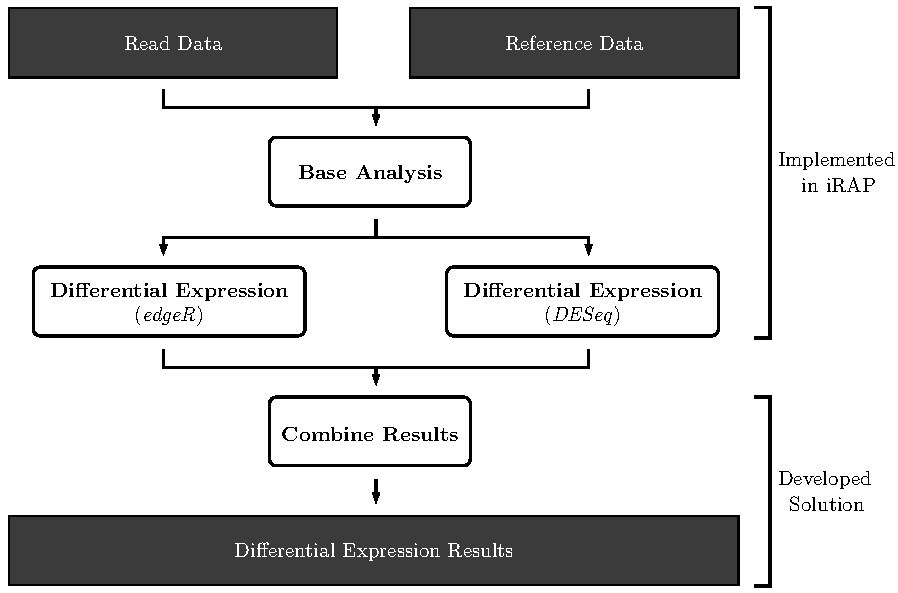
\includegraphics[]{tool1}
    \caption[Gene expression analysis pipeline workflow]{
      Gene expression analysis pipeline workflow.
    }
    \label{fig:tool1}
  \end{center}
\end{figure}

The next step is to sequentially execute differential expression analysis with
the chosen tools, in this case DESeq \cite{20979621} and edgeR
\cite{robinson2010edger}. The resulting files are kept until all tools are
executed. Note that there is no need for the analysis process to start from the
beginning every time a new tool is used, as iRAP can (in most cases) reuse the
results produced up until the point where a new tool is introduced.

After all tools are executed their results must be combined into a final list of
gene identifiers. This is done in an attempt to give researchers an higher level
of confidence in differential expression results. Note that this process is not
part of the iRAP analysis pipeline, and therefore a new tool must be developed.
Algorithm \ref{algo:combine} shows the basic process of combining the obtained
differential expression results. First, entries in every file must be filtered
by their \emph{p-value}\footnote{A \emph{p-value} is used to assert the
statistical significance of results. It represents the probability of obtaining
the same results as before in a new sample, given that the null hypothesis is
true \cite{goodman45dirty}.}, that must be inferior to a maximum threshold
($0.05$ by default). Then all entries in all files are compared with each other.
This produces an intersection of all files, in other words, a list of entries
that are present in all files.

\begin{algorithm}
  \emph{genes} = empty map\;
  \emph{files} = load all result files\;
  \ForEach{file \emph{in} files}{
    \ForEach{entry \emph{in} file}{
      \If{entry.pvalue $\leq$ 0.05}{
        increase gene count in \emph{genes}[\emph{entry.gene}]\;
      }
    }
  }
  \ForEach{gene, count \emph{in} genes}{
    \If{count $<$ number of files}{
      remove \emph{gene} from \emph{genes}
    }
  }
  write \emph{genes} to a file\;
  \BlankLine

  \caption[Combination of differential expression results]{
    Combination of differential expression results.
  }
  \label{algo:combine}
\end{algorithm}

\section{RNA Binding Protein Analysis Web Platform}

%\begin{Notes}
%- Present the name!\\
%- Minimal user input, infer most information.\\
%- Show analysis workflow (diagram).\\
%- Present standard RBP information.\\
%- Data set enrichment: show transcripts, proteins and their information
%(describe all info).\\
%- Two different types of clustering analysis, based on the used data and
%clustering criteria (describe algorithms, selection, etc.).\\
%- Briefly describe ERDA ILP analysis (and say it failed).\\
%\end{Notes}

The main objective of this system is to transform a complex, manually performed
analysis, into an automated workflow. The platform should require as little
information as possible from the user, inferring analysis parameters whenever
possible. It should also be able to automatically group genes (and proteins), to
reveal implied relationships between them that might be useful to experts. This
platform was named Protein Binding Site Finder (PBS Finder) and shall henceforth
be referred to by that name.

\subsection{Experimental Data}

The only data PBS Finder collects from the user is a list of gene (or
transcript) identifiers that should be analysed. These identifiers can be in one
of five different formats: \emph{Ensembl Gene}, \emph{Ensembl Transcript},
\emph{Entrez}, \emph{RefSeq} or \emph{GenBank} ( see Table \ref{tab:examples}).
Users can submit jobs with any combination of the previous types and use
identifiers from multiple species.

\begin{table}[!htb]
  \centering
  \begin{tabular}{{l} | {l}{l}}
    \textbf{\emph{Ensembl Gene}}        & ENSG00000224274 & ENSRNOG00000013536\\
    \textbf{\emph{Ensembl Transcript}}  & ENST00000003156 & ENSRNOT00000117589\\
    \textbf{\emph{Entrez}}              & 11245           & 66850\\
    \textbf{\emph{RefSeq}}              & NM\_001107622.1 & NM\_031098.1\\
    \textbf{\emph{GenBank}}             & U49845          & C35522\\
  \end{tabular}

  \caption[Examples of identifiers accepted by PBS Finder] {
    Two sets of examples of identifiers accepted by PBS Finder.
  }
  \label{tab:examples}
\end{table}

While PBS Finder can accept all these kinds of identifiers, internally the
analysis can only be started with \emph{Ensembl Gene} or \emph{Entrez}
identifiers, that map to Ensembl's and NCBI's pages, respectively. As such, the
identifiers must be first separated into different groups and converted. This
conversion is reviewed with more detail in Section \ref{sec:pbsworkflow}.

\subsection{User Information Management}

In order to use PBS Finder a new user must create an account, providing their
name and email, and choosing their authentication password. The account system
was implemented so that jobs could be associated with their creator in a cross
browser/system manner, in contrast with a typical cookie-based\footnote{Modern
websites sometimes need to save information about the user, for example
credentials. This data can be saved in the client machine, through the use of a
web browser cookie.} data persistence. This allows each user to list their own
jobs. Despite jobs being only directly accessible by their owner (creator), no
effort was made to deny users access to each other's jobs through the job's URL.
We believe that sharing results is an essential part of the investigation
process.

To create a new job the user provides a job description and an identifier list.
The identifier list is a newline-separated list (a single entry per line) of
unique identifiers for genetic information databases. In the current version
acceptable types of identifiers include Ensembl (both Gene and Transcript),
Entrez, RefSeq and GenBank. Users can submit jobs with any combination of the
previous types and use identifiers from multiple species. Upon job creation,
users can choose to be notified by email when the job finishes.

\subsection{Analysis Workflow}\label{sec:pbsworkflow}

PBS Finder is based on a three stage analysis model (Figure
\ref{fig:workflow2}): \emph{base analysis}, \emph{data set enrichment} and
\emph{clustering analysis}.

\begin{figure}[!htb]
  \begin{center}
    \leavevmode
    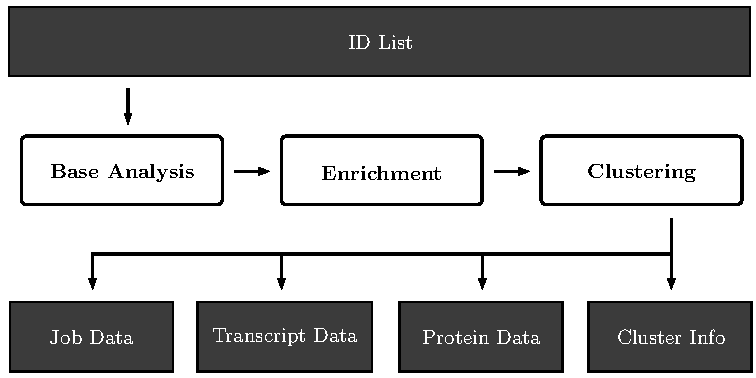
\includegraphics[width=0.75\textwidth]{workflow2}
    \caption[Simplified PBS Finder workflow]{
      Simplified PBS Finder workflow.
    }
    \label{fig:workflow2}
  \end{center}
\end{figure}

Base analysis comprises data set filtering, retrieval of basic gene and
transcript information and finding RBPs. The first released version of the
platform implemented only this stage of the analysis. It contains all the
information that is necessary to answer one of the base thesis problems.
However, further stages build on top of this information, bringing a more
valuable set of results to biologists.

In the enrichment stage additional information about every protein is retrieved.
This information is obtained from
UniProt\footnote{\url{http://www.uniprot.org}}, a web platform for curated
protein information. This stage was implemented in the second release of the
platform.

The clustering stage takes all the information collected in the previous stages
and uses it to perform clustering analysis. There are two types of clustering
analysis performed: \emph{clustering using RBP presence} and \emph{clustering
using RBP attributes}. The objective of this analysis is to uncover implicit
relationships in the collected data, that may be of use to biologists.

These stages are described in more detail in Chapter \ref{chap:implementation}.

\section{Tool Integration}

%\begin{Notes}
%- Complex pipeline with both tools.\\
%- Result reporting at each component.\\
%- Combined result reporting at the end.\\
%- Show integration diagram.\\
%\end{Notes}

In the designed solution both tools should be integrated, so that a user could
perform the complete analysis creating a unique analysis job. This would be
accomplished by using the interface of the RNA-Seq analysis pipeline as the
master (or main) interface for job creation. When the analysis completes, the
pipeline presents the preliminary results to the user and automatically launches
a PBS Finder analysis for the resulting gene identifier list. At this point the
RNA-Seq pipeline's interface should include a direct link to the created job in
PBS Finder. That link can then be used by the user to view the results of the
RBP localization analysis. Note that, while both tools are now integrated, the
results of both analyses are independent. As such, they can be
consulted/reviewed independently from each other, as if both had run separately.

\section{Chapter Conclusions}

%\begin{Notes}
%- Generic chapter conclusion.\\
%- Introduce next chapter of implementation details.\\
%\end{Notes}

In this chapter we reviewed the most important details about the design of the
proposed software solution (implementation details are described in Chapter
\ref{chap:implementation}). We presented the modular, two subsystem model, that
allows both tools to be used as standalone products, increasing the number of
their possible uses. Lastly, we talked about the general details of the
workflows of both tools, as well as the integration of those workflows.
